\section{Consistency as Reweighted Supervision}
\label{sec:analysis}

This section analyses the consistency term of a multi-view training loss. It shows that, when the
label is binary, a consistency term that draws one view toward the detached prediction of another
acts at every pixel as the supervised loss, rescaled by a factor that compares the errors of the
two views. The sign of this factor tells, pixel by pixel, whether the term helps or hurts, and
Section~\ref{sec:method} builds the weights of FCT on it.

\subsection{Notation}
\label{sec:notation}

Let $x\in\mathbb{R}^{H\times W\times 3}$ denote an image, $y\in\{0,1\}^{H\times W}$ its polyp mask,
and $f$ a segmentation network that maps $x$ to a logit map $z=f(x)\in\mathbb{R}^{H\times W}$; the
predicted probabilities are $p=\sigma(z)$, where $\sigma$ denotes the logistic function. Let $T_h$ and
$T_v$ denote the horizontal and vertical flips. Each flip is its own inverse, so the prediction for a
flipped view, brought back to the upright frame, is
\begin{equation}
z^{k}=T_k f(T_k x),\qquad k\in\{h,v\},
\label{eq:views}
\end{equation}
and the upright view gives $z^{o}=f(x)$. A flip-equivariant network satisfies $z^{h}=z^{v}=z^{o}$.
The flip gap of Section~\ref{sec:intro} measures departures from this equality on binary masks:
\begin{equation}
\Delta(x)=1-\frac{1}{2}\sum_{k\in\{h,v\}} D\big(\mathbf{1}[p^{o}>\tfrac12],\,\mathbf{1}[p^{k}>\tfrac12]\big),
\label{eq:flipgap}
\end{equation}
where $D$ denotes the Dice overlap of two masks and $\mathbf{1}[\cdot]$ the indicator function, applied
pixel by pixel.

At a pixel $i$, the error of a view is $e_i=|p_i-y_i|\in[0,1]$, and the view is correct at the
decision threshold of $\frac12$ if $e_i<\frac12$. We drop the index $i$ when a statement holds for
each pixel separately. A consistency term draws a view $s$ toward the prediction $p_t$ of a target
view $t$, which is detached, that is, treated as a constant. We write
\begin{equation}
\ell(z_s;q)=-q\log\sigma(z_s)-(1-q)\log\big(1-\sigma(z_s)\big)
\label{eq:bce}
\end{equation}
for the binary cross-entropy of the view's logit $z_s$ with a target $q\in[0,1]$. The consistency
term is $\ell(z_s;p_t)$ and the supervised loss is $\ell(z_s;y)$, and their gradients with respect to
the logit are
\begin{equation}
\frac{\partial\ell(z_s;p_t)}{\partial z_s}=p_s-p_t,\qquad
\frac{\partial\ell(z_s;y)}{\partial z_s}=p_s-y.
\label{eq:grads}
\end{equation}

\subsection{Consistency as an Adaptive Pixel Weight}
\label{sec:identity}

The two gradients in Eq.~\eqref{eq:grads} are parallel whenever the label is binary: the consistency
gradient is the supervised one, rescaled by how the errors of the two views compare.

\begin{proposition}
\label{prop:identity}
Let $y\in\{0,1\}$, $p_s,p_t\in[0,1]$ and $p_s\neq y$. Then
\begin{equation}
\frac{\partial\ell(z_s;p_t)}{\partial z_s}=\Big(1-\frac{e_t}{e_s}\Big)\frac{\partial\ell(z_s;y)}{\partial z_s},
\label{eq:identity}
\end{equation}
where $e_s=|p_s-y|$ and $e_t=|p_t-y|$ denote the errors of the view and of its target.
\end{proposition}

\begin{IEEEproof}
Because $y$ is $0$ or $1$, every $p\in[0,1]$ satisfies $p-y=(1-2y)|p-y|$: for $y=0$, $p-y=p$, and for
$y=1$, $p-y=-(1-p)$. Hence $p_s-p_t=(p_s-y)-(p_t-y)=(1-2y)(e_s-e_t)=(p_s-y)(1-e_t/e_s)$, where the last
step uses $(1-2y)e_s=p_s-y$ and $e_s>0$. Eq.~\eqref{eq:grads} completes the proof.
\end{IEEEproof}

The identity needs no assumption on the network or on the target's probability, only a binary
label, which places both errors on the same side of the target. It also holds for a squared-error
term on probabilities, whose gradient with respect to $p_s$ is again $p_s-p_t$. Summed over pixels
and differentiated with respect to the network parameters $\theta$, Eq.~\eqref{eq:identity} reads
\begin{equation}
\nabla_\theta\sum_i \ell(z_{s,i};p_{t,i})=\sum_i \omega_i\,\nabla_\theta\,\ell(z_{s,i};y_i),
\qquad \omega_i=1-\frac{e_{t,i}}{e_{s,i}},
\label{eq:weights}
\end{equation}
with the weights $\omega_i$ held constant. A consistency term is thus a supervised loss with
per-pixel weights, and some of these weights are negative.

When the view is also supervised, the two terms add. With a cross-entropy supervised term of weight
$\beta$ and a consistency term of weight $\gamma$, the gradient on the view's logit is
\begin{equation}
\big(\beta+\gamma\,\omega\big)\,(p_s-y),
\label{eq:combined}
\end{equation}
so the consistency term changes only how much each pixel's supervised gradient counts. Under full
supervision, it brings no information beyond the label: it acts as an adaptive pixel weight, as
focal loss~\cite{lin2017focal} and the structure loss~\cite{wei2020f3net} do, but set by how the
pixel's error in one view compares with its error in another.

\begin{corollary}[Lag condition]
\label{cor:lag}
Under the conditions of Proposition~\ref{prop:identity}, a gradient step on $\ell(z_s;p_t)$ moves the
view's probability toward the label if $e_t<e_s$, away from it if $e_t>e_s$, and not at all if
$e_t=e_s$.
\end{corollary}

\begin{IEEEproof}
A step of size $\eta$ changes the logit by $-\eta(p_s-p_t)=-\eta\,\omega\,(p_s-y)$, by
Eq.~\eqref{eq:identity}. The supervised step $-\eta(p_s-y)$ moves $p_s$ toward $y$ because $\sigma$ is
increasing, and $\omega>0$ if and only if $e_t<e_s$.
\end{IEEEproof}

To first order, the step lowers the view's error by $\eta\,\sigma'(z_s)(e_s-e_t)$, so we call $e_s-e_t$
the movement toward the label. Fig.~\ref{fig:pull}(a) maps it over the two errors. Below the diagonal,
the view lags behind its target, and the term helps. Above it, the view leads, and the term hurts, in
two ways. Where the target is wrong and the view right ($e_s<\frac12<e_t$), the term drives a correct
pixel toward a misclassification, with a strength $e_t-e_s$ that can approach that of a full supervised
step. Where both are right ($e_s<e_t<\frac12$), the term only lowers the view's confidence, and it stops
when the view reaches its target, on the correct side of the threshold.

\begin{figure*}[t]
\centering
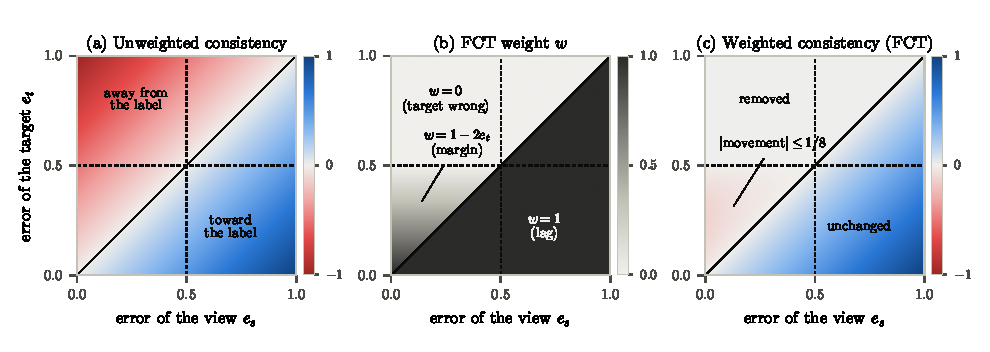
\includegraphics[width=0.96\textwidth]{figures/fig_pull.pdf}
\caption{Effect of a consistency term on the error of a view at one pixel, as a function of the view's
error $e_s$ and the error $e_t$ of its detached target (Proposition~\ref{prop:identity}); dashed lines
mark the decision threshold. (a)~Without a weight, the term moves the view away from the label wherever
the view is the closer of the two, even toward a wrong target (top left). (b)~The FCT weight of
Eq.~\eqref{eq:weight}. (c)~With it, every movement toward the label is kept, every movement away from
the label toward a wrong target is removed, and the remaining movements away from the label are
bounded by $1/8$.}
\label{fig:pull}
\end{figure*}

In semi-supervised learning, no label separates the two cases, so the views are drawn together alike.
Under full supervision, the label separates them at every pixel: the term can keep its full weight
where the view lags behind its target, and elsewhere act only where it cannot reverse a correct
decision. Section~\ref{sec:method} turns this rule into the weights of the FCT loss.
